% In the header are the basic settings of the document
\documentclass[12pt,a4paper]{article} % 12-point font, A4 paper
\usepackage[utf8]{inputenc} 
% \usepackage[ngerman]{babel} % Adjusts all automatic texts. 
\usepackage[english]{babel} % Use this variant if you are writing a paper in English.

\parindent=0cm
\parskip=0.3cm
\linespread{1.5}

% A few standard packages. One must know exactly what they are needed for...
\usepackage{amsmath}
\usepackage{amsfonts}
\usepackage{amssymb}
\usepackage{pdfpages}
\usepackage{hyperref}
\usepackage{csquotes}
\usepackage{graphicx}

\graphicspath{{images/}}

% for chessboards
% \usepackage{xskak,chessboard}

\usepackage[
    backend=biber,
    style=apa,
    sortlocale=de_DE,
    natbib=true,
    url=false,
    doi=false,
    sortcites=true,
    sorting=nyt,
    isbn=false,
    hyperref=true,
    backref=false,
    giveninits=false,
    eprint=false]{biblatex}
\addbibresource{references/bibliography.bib}

% Information for the title page
\title{Example for a Matura Thesis}
\date{\today}
\author{Susy Muster}

% The beginning of the document
\begin{document}

\maketitle % Here the title page with the above information is inserted. If you want to create a more "artistic" title page with another program, you can insert it here. For this, you must place the title page in the same directory (e.g., named TitelseiteMA2016.pdf) in pdf format and it will be inserted with the command
% \includepdf{TitelseiteMA2016}

\newpage % A new page begins...
\tableofcontents % Here the table of contents is automatically inserted. Note: Changes are only visible after the second compilation.

\newpage

\section{Structure}

A section is created with this command:
\begin{verbatim}
\section{Introduction}
\end{verbatim}

It looks like this:

% The basic structure of a paper:
\section{Introduction}
Here comes text\ldots 

Subsections are presented like this:

\begin{verbatim}
\subsection{Sources and Citations}
\end{verbatim}

and look like this:

\subsection{Sources and Citations}

% A new paragraph begins with a blank line

If you want to reference a source, use the \verb|\citet{}| or \verb|\citep{}| command \citep{example}. You can also cite a second source: “Life finds a way” \citep{buch2}.

\citet{example} says \dots

\newpage

\section{Images}

Images/graphics are inserted with the following command:

\begin{verbatim}
\begin{figure}[h]
\centering 
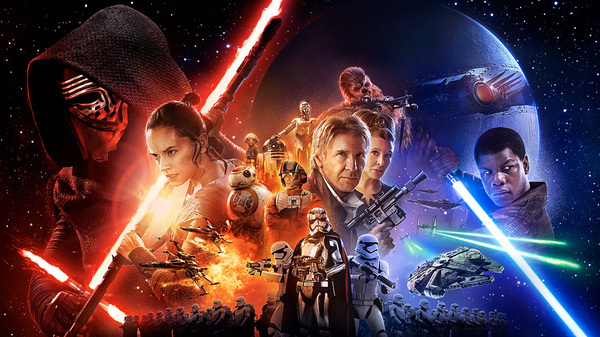
\includegraphics[width=0.5\textwidth]{star_wars.jpeg}
\caption{A first image \cite{sw16}}
\end{figure}
\end{verbatim}

The \verb|figure| environment draws an image, \verb|[h]| means that the graphic should be embedded in the text as close as possible.

It looks like this:

\begin{figure}[h] % The "figure" environment 
\centering % This centers the image
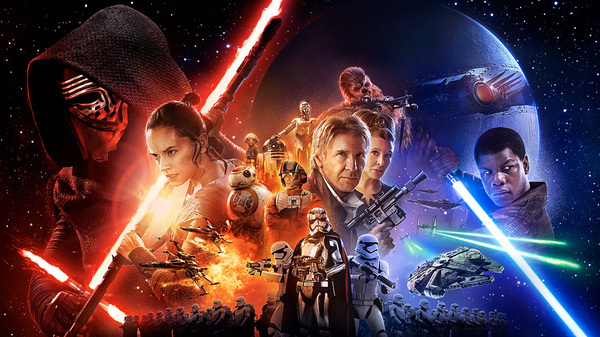
\includegraphics[width=0.5\textwidth]{star_wars.jpeg} % Here an image is inserted, which is located in the same directory. It is resized to fit half the text width.
\caption{A first image \citep{star-wars}}
\end{figure}

Images automatically appear in the list of figures.

\newpage

% \section{Chessboards}
% Chessboards with specific positions can be specified in the FEN notation (Forsyth-Edwards Notation (FEN) or in the extended form (X-FEN) is a short notation to describe any chess position. \cite{fen-wiki}):

% \begin{verbatim}
% \begin{figure}[h]
% \centering
% \chessboard[setfen=1n1Rkb1r/p4ppp/4q3/4p1B1/4P3/8/PPP2PPP/2K5 b k - 1 17]
% \caption{Checkmate! (Morphy vs. Karl von Braunschweig and Count Isoard, 1858)}
% \end{figure}
% \end{verbatim}

% It looks like this:
% \setchessboard{showmover=false}

% \begin{figure}[h]
% \centering
% \chessboard[setfen=1n1Rkb1r/p4ppp/4q3/4p1B1/4P3/8/PPP2PPP/2K5 b k - 1 17]
% \caption{Checkmate! (Morphy vs. Karl von Braunschweig and Count Isoard, 1858)}
% \end{figure}

% \newpage

% Moves can be drawn with the command \verb|markmoves|:

% \begin{verbatim}
% \begin{figure}[h]
% \centering
% \chessboard[smallboard,
% setpieces={Ra1,Rh1,Ke1,ke8,rh8,ra8,Ne6,bb4},
% arrow=to,linewidth=0.2ex,
% pgfstyle=knightmove,
% shortenstart=0.4em,
% color=red!80,
% markmoves={e6-d8,e6-f8},
% pgfstyle=straightmove,
% shortenstart=0.4em,
% color=red!80,
% markmoves={b4-e1},
% ]
% \caption{No castling possible}
% \end{figure}
% \end{verbatim}

% \begin{figure}[h]
% \centering
% \chessboard[smallboard,
% setpieces={Ra1,Rh1,Ke1,ke8,rh8,ra8,Ne6,bb4},
% arrow=to,linewidth=0.2ex,
% pgfstyle=knightmove,
% shortenstart=0.4em,
% color=red!80,
% markmoves={e6-d8,e6-f8},
% pgfstyle=straightmove,
% shortenstart=0.4em,
% color=red!80,
% markmoves={b4-e1},
% ]
% \caption{No castling possible}
% \end{figure}

% \newpage

\section{Conclusions}
\newpage

% Here begins the appendix
\appendix
\section{Appendix}
\newpage

\section{List of Figures}
\listoffigures

\newpage

\printbibliography

\end{document}
